
%%% Local Variables:
%%% mode: latex
%%% TeX-master: t
%%% End:

\chapter{基于AS编址的互联网FIB表的生成与压缩情况评估}
\label{cha:compression}
\section{引言}
本章将详细介绍当前网络下FIB表的生成过程以及在新型编址方案CABA下采用基于ASN的BGP协议时FIB表的情况,通过对比评估新型编址环境下路由的可扩展性。
\section{数据集介绍}
实验的数据集来自Oregon大学的Route Views\onlinecite{bgpdata}工程搜集的BGP数据。进入FTP下载页面,选择13台路由器(路由器的名称为: perth, isc, linx, sydney, wide, eqix, saopaulo, nwax, telxatl, jinx, soxrs, sg, kixp),获取其2015年4月3日0点的全局路由表。

\section{当前网络下的FIB表}
\label{sect:fibtab}
\begin{enumerate}
\item 从Oregon大学的Route Views\onlinecite{bgpdata}下载13台路由器的RIB数据,下载的原始数据是二进制格式,需要工具来解析。
\item 使用libbgpdump\onlinecite{libbgpdump}解析二进制文件。需要从github上下载libbgpdump 的源代码,先执行configure,然后执行make即可生成bgpdump可执行文件,之后通过$./bgpdump -M -O outputfile inputfile$ 命令获取解析后的文件,使用M参数简化路由表项(如:TABLE\_DUMP\_V2|03/31/15 02:00:00|A|206.126.236.120|41095|0.0.0.0/0|41095 3356|IGP)。
\item 相同前缀在RIB表中可能有多条路由信息,但不考虑多路由机制,FIB表中存储的是该前缀的最优路由信息。评价最优路径有两个原则:路径的长度要最短,当路径长度相同的时候,选择下一跳自治系统号最小的路由信息。编写函数,将13台路由器的RIB表转换成FIB 表。
\end{enumerate}

\section{基于AS新型编址下FIB表的设计与生成}
本章节将详细介绍基于AS新型编址下FIB表设计与生成的关键技术和增量部署的过程。
\subsection{关键技术}
将现有网络中的FIB表转换成基于AS新型编址CABA下的FIB表的主要过程如下所示:
\begin{enumerate}
\item 一个自治系统可能向外宣布多条前缀,在CABA编制下一个自治系统只需要向外宣布一条前缀。我们将当前网络中的FIB表中数据进行分析,每一项数据找到宣布这条前缀的源ASN,如果两个不同IP前缀的源ASN相同,则证明这两个不同IP前缀是由同一个自治系统宣告出来。找出同一个自治系统宣布所有前缀的表项,将其前缀替换成CABA 格式的IPv6$/$40前缀。前8位为保留位,选择IANA 未使用的地址段10;之后32位为源自治系统的ASN。
\item 因为在现有网络中的FIB表中,有些前缀是由聚合的AS集合宣告的,你并不知道这些前缀究竟是由哪个自治系统向外宣告的。经过对这13台路由器的FIB 表中聚合AS集合数目大于1的表项进行统计,每个路由器约有50万条数据的FIB表中约有50条这样的表项,不足万分之一的数据。为了保证用CABA编址格式下的前缀替换原有前缀的准确性,我们舍弃这不足万分之一的聚合AS集合数目大于1的表项。
\item 替换前缀结束后,在FIB表中同一个自治系统向外公布了一条前缀,但到达这条前缀有多条路径,我们选择最优路径保留下来,其余舍弃。评价最优路径依旧遵循两个原则:路径的长度要最短,当路径长度相同的时候,选择下一跳自治系统号最小的路由信息。编写函数,将13台路由器的RIB表转换成FIB 表。
\end{enumerate}

\subsection{增量部署}
现今互联网架构和规模已经很大,协议和策略已经很完备,并且渗透到经济社会生活的方方面面,将基于AS的新型编址CABA完全部署到互联网上是不现实的,所以需要进行增量部署。本章节对两种增量部署方案的结果进行了评估,两种增量部署的方案如下:
\begin{itemize}
\item 我们得到13台路由器CABA编址下的FIB表,统计每张表的表项,表示该全局路由表中自治系统的个数。

    \begin{table}[h]
    \centering
    \caption{路由器中AS的数目}
    \label{tab:routeasnum}
        \begin{tabular}{|c|c|}
            \hline
            路由器名称 & AS数目 \\ \hline
            perth & 913 \\ \hline
            isc   & 50034 \\ \hline
            linx & 49934  \\ \hline
            kixp & 146 \\ \hline
            sydney& 50059  \\ \hline
            wide  & 49882  \\ \hline
            eqix  & 50002  \\ \hline
            saopaulo & 49953 \\ \hline
            nwax  & 49950   \\ \hline
            telxatl  & 49968 \\ \hline
            jinx  & 49685 \\ \hline
            soxrs  & 11880  \\ \hline
            sg    & 49939 \\  \hline
        \end{tabular}
    \end{table}

从上表\ref{tab:routeasnum}可以看出perth、soxrs、kixp这三台路由器可能是边界路由器,没有全局路由表的所有信息,所以我在剩余的10台路由器中随机一台路由器的FIB表,从而获取增量部署时所有的ASN,随机路由器的结果为名为saopaulo路由器。
\item 根据saopaulo路由器当前网络下的FIB表的数据,提取所有的ASN以及统计其自治系统宣布的前缀数目,每一个表项可以找到发布的前缀以及源自治系统的ASN。
\item 本章设计了三种部署方案:随机部署和根据宣告前缀数目部署。

    \begin{itemize}
        \item 随机部署:获取saopaulo路由器的当前网络下FIB表数据中前缀对应的所有ASN,随机选取所有ASN的20\%,40\%,60\%,80\%,100\%作为部署CABA编址的自治系统。
        \item 根据宣告前缀数目部署:获取saopaulo路由器的当前网络下FIB表数据中前缀对应的所有源ASN以及同一个自治系统向外宣布的前缀数目,将ASN 根据宣告前缀的数目由大到小排序,选取排序后的20\%,40\%,60\%,80\%,100\%。理论上当增量部署的程度相同时,部署宣告前缀越多的自治系统,路由表的压缩比例越多。
        \item 部署tier1层级的自治系统,tier1为互联网层级结构的最顶层,tier1层级的自治系统不论到达互联网的任何地方,都不需要支付转发和暂存等费用\cite{tier1}。
    \end{itemize}

\end{itemize}
\section{FIB表压缩情况的评估}
本章节显示FIB表的压缩结果以及对结果进行分析。
\subsection{压缩结果}
在增量部署的情况下,得到FIB表的原始数据:

\begin{table}[h]
    \centering
    \caption{随机部署:FIB压缩原始数据}
    \label{tab:origindata}
        \begin{tabular}{|c|c|c|c|c|c|c|}
            \hline
            路由器名称 & 当前网络FIB数目 & 部署20\% &部署40\% &部署60\% &部署80\% &部署100\% \\ \hline
            perth    & 8476   & 7551   & 4189   & 3360   & 3045   & 913     \\ \hline
            isc      & 573459 & 464036 & 353547 & 257451 & 170197 & 50034    \\ \hline
            linx     & 562937 & 455543 & 347739 & 253285 & 164897 & 49934     \\ \hline
            kixp     & 2329   & 2059   & 1255   & 1016   & 298    & 146        \\ \hline
            sydney   & 572895 & 462372 & 351338 & 255924 & 165075 & 50059       \\ \hline
            wide     & 558015 & 452474 & 345574 & 251150 & 165999 & 49882        \\ \hline
            eqix     & 561370 & 454054 & 347624 & 251743 & 164012 & 50002         \\ \hline
            saopaulo & 575586 & 466723 & 357205 & 258361 & 167807 & 49953          \\ \hline
            nwax     & 558075 & 451568 & 346512 & 250927 & 162610 & 49950           \\ \hline
            telxatl  & 558182 & 451432 & 346063 & 250583 & 164080 & 49968            \\ \hline
            jinx     & 536466 & 432900 & 334158 & 241083 & 157437 & 49685             \\ \hline
            soxrs    & 38037  & 32766  & 26930  & 22203  & 17930  & 11880              \\ \hline
            sg       & 557282 & 450476 & 345647 & 249168 & 162759 & 49939               \\ \hline
        \end{tabular}
\end{table}


\begin{table}[h]
    \centering
    \caption{根据宣告前缀数目部署:FIB压缩原始数据}
    \label{tab:prefixorigindata}
        \begin{tabular}{|c|c|c|c|c|c|c|}
            \hline
            路由器名称 & 当前网络FIB数目 & 部署20\% &部署40\% &部署60\% &部署80\% &部署100\% \\ \hline
            perth    & 8476   & 1977   & 1143   & 935   & 916   & 913     \\ \hline
            isc      & 573459 & 107546 & 65913  & 51985 & 50157 & 50034    \\ \hline
            linx     & 562937 & 106499 & 65513  & 5177  & 49984 & 49934     \\ \hline
            kixp     & 2329   & 306    & 208    & 181   & 160   & 146        \\ \hline
            sydney   & 572895 & 107023 & 65748  & 51974 & 50126 & 50059       \\ \hline
            wide     & 558015 & 105825 & 65335  & 51724 & 49955 & 49882        \\ \hline
            eqix     & 561370 & 106529 & 65531  & 51828 & 50049 & 50002         \\ \hline
            saopaulo & 575586 & 575586 & 65382  & 51689 & 49953 & 49953          \\ \hline
            nwax     & 558075 & 106092 & 65372  & 51745 & 49979 & 49950           \\ \hline
            telxatl  & 558182 & 106262 & 65465  & 51788 & 50013 & 49968            \\ \hline
            jinx     & 536466 & 99756  & 62580  & 51125 & 49739 & 49685             \\ \hline
            soxrs    & 38037  & 15384  & 12858  & 12003 & 11881 & 11880              \\ \hline
            sg       & 557282 & 106131 & 65447  & 51749 & 49971 & 49939               \\ \hline
        \end{tabular}
\end{table}

\begin{figure}
  \centering
  % Requires \usepackage{graphicx}
  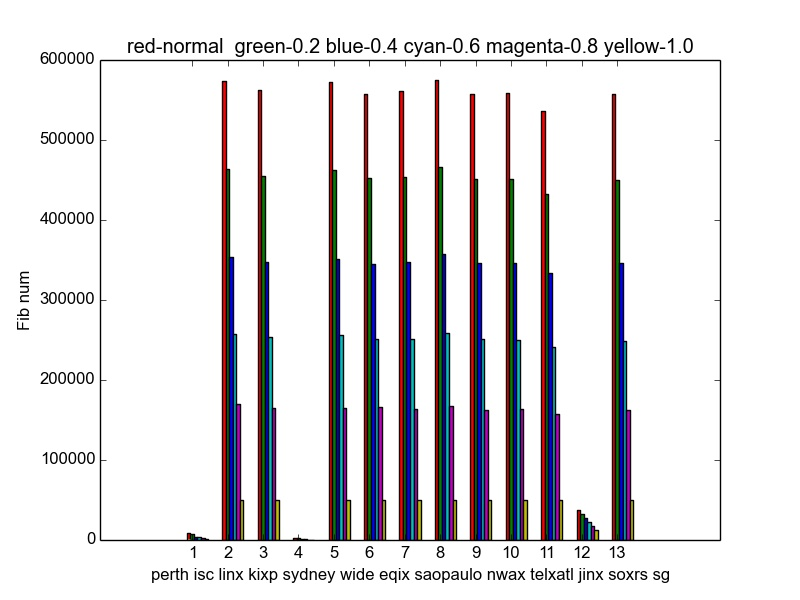
\includegraphics[width=\textwidth]{2}
  \caption{随机部署:FIB表项数目}
  \label{fig:2}
\end{figure}

\begin{figure}
  \centering
  % Requires \usepackage{graphicx}
  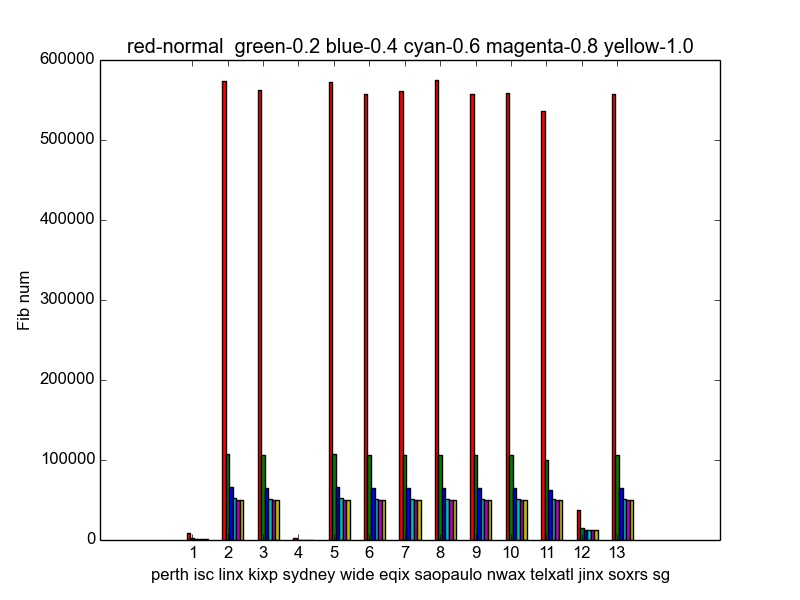
\includegraphics[width=\textwidth]{3}
  \caption{根据宣告前缀部署:FIB表项数目}
  \label{fig:3}
\end{figure}

本节我们首先看到随机部署\ref{tab:origindata}和根据宣告前缀数目部署\ref{tab:prefixorigindata}两种情况下路由表的压缩情况。从数据能很明显看到在随机部署中,FIB 表项随着部署比例的线性增加而线性减少,如图\ref{fig:2},而根据宣告前缀数目部署中FIB表项在部署比例为20\%时,大幅度减少,之后缓慢减少,如图\ref{fig:3}。说明一个自治系统向外宣告前缀越多,该自治系统采用CABA编址后,对FIB表的压缩贡献越大。由此我们可以设想,如果将Tier1的自治系统全部部署CABA编址,对FIB表的压缩程度也应该会很大,之后通过实验获得了下图的数据。

\begin{table}[h]
    \centering
    \caption{部署tier1自治系统:FIB压缩原始数据}
    \label{tab:tieronefibdata}
    \begin{tabular}{|c|c|c|c|}
    \hline
            路由器名称 & 当前网络FIB表项数目 & 部署tier1后表项数目 & 部署tier1后减少表项数目\\ \hline
            perth    & 8476   & 8476   & 0  \\ \hline
            isc      & 573459 & 562564 & 10895   \\ \hline
            linx     & 562937 & 551601  & 11336   \\ \hline
            kixp     & 2329   & 2329   & 0        \\ \hline
            sydney   & 572895 & 562573 & 10322      \\ \hline
            wide     & 558015 & 547127 &  10888         \\ \hline
            eqix     & 561370 & 551601 & 9769        \\ \hline
            saopaulo & 575586 & 564435 & 11151       \\ \hline
            nwax     & 558075 & 548597  &     9478     \\ \hline
            telxatl  & 558182 & 548524   &  9658      \\ \hline
            jinx     & 536466 & 527490    &     8976    \\ \hline
            soxrs    & 38037  & 37643      &  394   \\ \hline
            sg       & 557282 & 547893    & 9389\\ \hline
    \end{tabular}
\end{table}

\begin{table}
    \centering
    \caption{tier1自治系统号}
    \label{tab:tier1asn}
    \begin{tabular}{|c|c|c|c|c|c|}
    \hline
    174 & 209 & 286 & 701 & 1239 & 1299 \\ \hline
    2828 & 2914 & 3257 & 3320 & 3356 & 5511 \\ \hline
    6453 & 6461 & 6762 & 7018 & 12956 & - \\ \hline
    \end{tabular}
\end{table}

tier1的自治系统号来源于CAIDA官网上的数据\onlinecite{caidaasdata},下载20150201时间的AS关系数据,在其关系数据里面有tier1 的ASNs见表\ref{tab:tier1asn},部署这些自治系统,我们可以看到部署17个自治系统,核心网络FIB 表的表项可以减少约1万条,约占当前网络FIB表50万表项的2\%, 验证了我们的设想。

\subsection{结果分析}
本节对三中部署方案的FIB表的压缩率进行计算绘图说明其变化趋势。

\begin{table}[h]
    \centering
    \caption{随机部署:FIB压缩率}
    \label{tab:origindatarate}
        \begin{tabular}{|c|c|c|c|c|c|c|}
            \hline
            路由器名称 & 当前网络FIB数目 & 部署20\% &部署40\% &部署60\% &部署80\% &部署100\% \\ \hline
            perth    & 8476   & 0.10913   & 0.50578  & 0.60359   & 0.64075   & 0.89228     \\ \hline
            isc      & 573459 & 0.19081 & 0.38348 & 0.55106 & 0.70321 & 0.91275    \\ \hline
            linx     & 562937 & 0.19077 & 0.38228 & 0.55007 & 0.70708 & 0.91130     \\ \hline
            kixp     & 2329   & 0.11593   & 0.46114   & 0.56376   & 0.87205    & 0.93731        \\ \hline
            sydney   & 572895 & 0.19292 & 0.38673 & 0.55328 & 0.71186 & 0.91262       \\ \hline
            wide     & 558015 & 0.18914 & 0.38071 & 0.54992 & 0.70252 & 0.91061        \\ \hline
            eqix     & 561370 & 0.19117 & 0.38076& 0.55156 & 0.70784 & 0.91093         \\ \hline
            saopaulo & 575586 & 0.18913 & 0.37941 & 0.55113 & 0.70846 & 0.91321          \\ \hline
            nwax     & 558075 & 0.19085 & 0.37909 & 0.55037 & 0.70862 & 0.91050           \\ \hline
            telxatl  & 558182 & 0.19125 & 0.38002 & 0.55107 & 0.70605 & 0.91048            \\ \hline
            jinx     & 536466 & 0.19305 & 0.37711 & 0.55061 & 0.70653 & 0.90738             \\ \hline
            soxrs    & 38037  & 0.13858  & 0.29201  & 0.41628  & 0.52862  & 0.68767            \\ \hline
            sg       & 557282 & 0.19166 & 0.37976 & 0.55289 & 0.70794 & 0.91039              \\ \hline
        \end{tabular}
\end{table}

由图\ref{tab:origindatarate}可以看出,随机部署环境下,FIB 表压缩率(FIB表减少表项\/FIB表原有表项)随着部署比例的线性增加而线性增加,明显的趋势图如\ref{fig:2rate}。

\begin{table}[h]
    \centering
    \caption{根据宣告前缀数目部署:FIB压缩率}
    \label{tab:prefixorigindatarate}
        \begin{tabular}{|c|c|c|c|c|c|c|}
            \hline
            路由器名称 & 当前网络FIB数目 & 部署20\% &部署40\% &部署60\% &部署80\% &部署100\% \\ \hline
            perth    & 8476   & 0.76675   & 0.86515   & 0.88969   & 0.89193   & 0.89228      \\ \hline
            isc      & 573459 & 0.81246 & 0.88506  & 0.90935 & 0.91254 & 0.91275    \\ \hline
            linx     & 562937 & 0.81082 & 0.88362 & 0.90803  & 0.91121 & 0.91130     \\ \hline
            kixp     & 2329   & 0.86861    & 0.91069    & 0.92228   & 0.93130   & 0.93731        \\ \hline
            sydney   & 572895 & 0.81319 & 0.88523  & 0.90928 & 0.91250 & 0.91262       \\ \hline
            wide     & 558015 & 0.81035 & 0.88292  & 0.90731 & 0.91048 & 0.91061        \\ \hline
            eqix     & 561370 & 0.81023 & 0.88327  & 0.90768 & 0.91084 & 0.91093         \\ \hline
            saopaulo & 575586 & 0.81466 & 0.88641  & 0.91020 & 0.91321 & 0.91321          \\ \hline
            nwax     & 558075 & 0.80990 & 0.88286  & 0.90728 & 0.91044 & 0.91050           \\ \hline
            telxatl  & 558182 & 0.80963 & 0.88272  & 0.90722 & 0.91040 & 0.91048            \\ \hline
            jinx     & 536466 & 0.81405  & 0.88335  & 0.90470 & 0.90728 & 0.90738             \\ \hline
            soxrs    & 38037  & 0.59555  & 0.66196  & 0.68444 & 0.68765 & 0.68767              \\ \hline
            sg       & 557282 & 0.80956 & 0.88256  & 0.90714 & 0.91033 & 0.91039               \\ \hline
        \end{tabular}
\end{table}

由图\ref{tab:prefixorigindatarate}可以看出,根据宣告前缀数目部署环境下,FIB 表压缩率(FIB表减少表项\/FIB表原有表项)在部署比例为20\%的情况下上升到很大的值,之后随着部署比例的线性增加二缓慢增加,明显的趋势图如\ref{fig:3rate}。

\begin{table}[h]
    \centering
    \caption{部署tier1自治系统:FIB率}
    \label{tab:tieronefibdatarate}
    \begin{tabular}{|c|c|c|c|}
    \hline
            路由器名称 & 当前网络FIB表项数目 & 部署tier1后FIB压缩率 & 部署tier1后减少表项数目\\ \hline
            perth    & 8476   & 0.0   & 0  \\ \hline
            isc      & 573459 & 0.01900 & 10895   \\ \hline
            linx     & 562937 & 0.01978  & 11336   \\ \hline
            kixp     & 2329   & 0.0   & 0        \\ \hline
            sydney   & 572895 & 0.01802 & 10322      \\ \hline
            wide     & 558015 & 0.01951 &  10888         \\ \hline
            eqix     & 561370 & 0.01740 & 9769        \\ \hline
            saopaulo & 575586 & 0.01937 & 11151       \\ \hline
            nwax     & 558075 & 0.01698  &     9478     \\ \hline
            telxatl  & 558182 & 0.01730  &  9658      \\ \hline
            jinx     & 536466 &   0.01673   &     8976    \\ \hline
            soxrs    & 38037  & 0.01036     &  394   \\ \hline
            sg       & 557282 & 0.01685    & 9389\\ \hline
    \end{tabular}
\end{table}

属于tier1的自治系统有17个,部署之后,对于现在的约50万的FIB表数据,可以压缩1万的表项,非常多了,占到了压缩比例的2\%,如图\ref{tab:tieronefibdatarate}但是17个自治系统相对于目前网络50000个自治系统只占0.034\%,是2\%的1\/58,也就是说部署一个tier1的自治系统相当于部署58个普通层级的自治系统。

\begin{figure}
  \centering
  % Requires \usepackage{graphicx}
  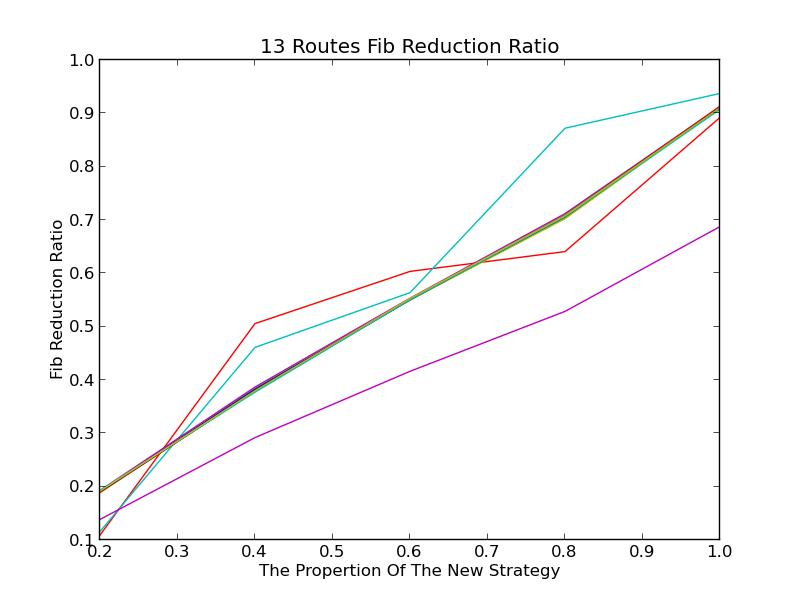
\includegraphics[width=\textwidth]{2rate}
  \caption{随机部署:FIB表项数目}
  \label{fig:2rate}
\end{figure}

\begin{figure}
  \centering
  % Requires \usepackage{graphicx}
  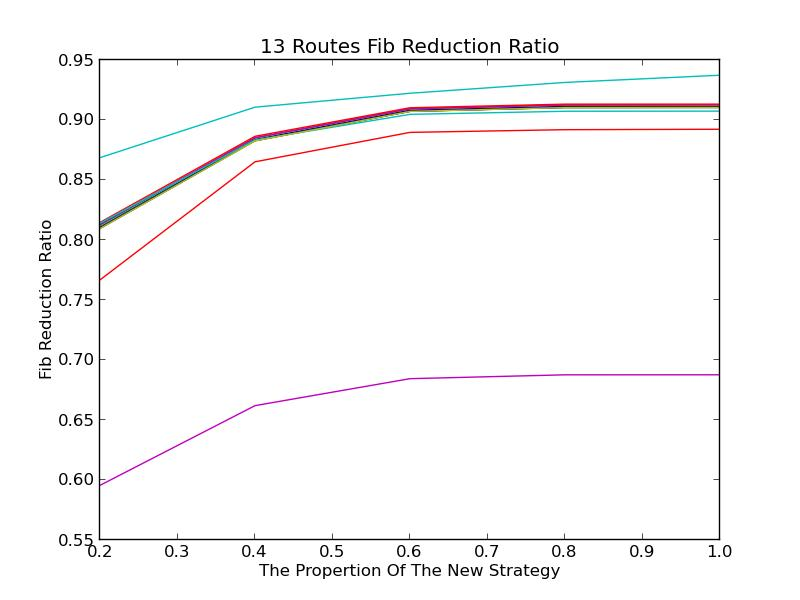
\includegraphics[width=\textwidth]{3rate}
  \caption{根据宣告前缀部署:FIB表项数目}
  \label{fig:3rate}
\end{figure}

\section{小结}
总体来看,在全部部署的情况下,FIB表的表项数目是现网络环境下FIB表表项的1\/10,增量部署的情况下,FIB表表项的压缩情况与部署自治系统向外宣布的前缀数目相关,部署自治系统向外宣告的前缀数目越多,FIB表表项的压缩情况越好。所以,我们在增量部署CABA编址时,可以考虑层级较高的自治系统和向外公布前缀较多的自治系统,这样对全局FIB的压缩作用会比较明显。
